%!TEX root = ./binder.tex
%-------------------------------------------------------------------------------
\section{Implementation}
%-------------------------------------------------------------------------------

We implemented our approach in the tool {\bcov}.
Our tool accepts an ELF module (executable or shared library) as input.
It starts with a set of module-level analyses such as reading function definitions, parsing CFI records, and building the call graph.
Our non-return analysis implementation is similar to~\cite{Meng:ISSTA2016}.
We omit the details as they are not part of our core contribution.

Then, {\bcov} moves to function-level analyses such as building the CFG (including jump tables), dominator trees, and superblock dominator graph.
Probes are determined based on the instrumentation policy set by the user.
{\bcov} can be used for patching or coverage reporting.
The latter mode requires a data file dumped from a patched module.
The instrumentation policy used for coverage reporting must match the one used for patching. 

We implemented the modern SEMI-NCA dominator tree algorithm~\cite{Georgiadis2005} and Tarjan's classical SCC algorithm.
We used \textsf{capstone}~\cite{CapstoneEngine} for disassembly and implemented a wrapper around \textsf{unicorn}~\cite{UnicornEngine} for microexecution.
In total, this required about 17,000 LoC in C++ (testing code excluded).
The run-time library \textsf{bcov-rt} is implemented in C in $\sim$250 LoC.


%-------------------------------------------------------------------------------
\section{Evaluation}
\label{sec:evaluation}
%-------------------------------------------------------------------------------

Our evaluation is guided by the following research questions:

\begin{description}
    \itemsep-.1em
    \item[RQ1] Can {\bcov} transparently scale to large real-world binaries?
    \item[RQ2] What is the instrumentation overhead in terms of performance, memory, and file size?        
    \item[RQ3] Have we pushed the state of the art in jump table analysis?    
    \item[RQ4] To what extent can {\bcov} provide better efficiency in comparison to its direct alternatives, namely, DBI tools?    
    \item[RQ5] Can {\bcov} accurately report binary-level coverage?    

\end{description}

For evaluation, we selected eight modules from popular open-source packages offering diverse functionality.
They are summarized in Table~\ref{tab:selected-benchmarks}.
We compiled each module using four compilers in three different build types.
Specifically, we used the compilers \textsf{gcc-5.5}, \textsf{gcc-7.4}, \textsf{clang-5.0}, and \textsf{clang-8.0}.
This gives us a representative snapshot of the past three years of developments in \textsf{gcc} and \textsf{clang} respectively.
The build types are \textsf{debug}, \textsf{release}, and \textsf{lto}.
The latter refers to link-time optimizations.
Compiler optimizations were disabled in \textsf{debug} builds and enabled in \textsf{release} and \textsf{lto} builds.
Enabled optimizations depend on the default options of their respective package which can  be at levels \texttt{O2} or \texttt{O3}.



This results in 12 versions of each module and a total of 95 binaries.
\footnote{Compiling \textsf{llc} with \textsf{gcc-5.5} in \textsf{lto} build resulted in a compiler crash.}
Our tool was capable of patching 88 binaries without modifying the build system.
However, we had to modify the linker script in 7 instances where relocating ELF segment headers was not possible. 
We instructed the linker to leave 112 bytes, which is enough for our segment headers, after the original segment headers.
This change is small affecting only one line in the linker script.
The \mbox{\textsf{bcov-rt}} runtime was injected using the LD\_PRELOAD mechanism.
All experiments were conducted on an Ubuntu 16.04 PC with Intel\textsuperscript{\textregistered} i7-6700 CPU and 32GB of RAM.

\subsection*{RQ1. Scalability and Transparency}
Our choice of subjects directly supports our claim regarding scalability.
Figure~\ref{fig:code-size-comp} shows a comparison in terms of code size relative to \textsf{objdump}, a commonly used subject in binary analysis research.
Code size is measured using the popular \texttt{size} utility.
Note that {\bcov} can analyze and patch our largest subject, \textsf{llc}, in $\sim$30 seconds.
In our experiments, we used {\bcov} to instrument all functions  available in the \texttt{.text} section.
More than $1.6\times10^6$ functions have been instrumented across 95 binaries.
The policies leaf-node and any-node have been applied separately, i.e., subjects were instrumented twice.


\begin{table}[t!]
	\centering
	\setlength\tabcolsep{4pt}
	\small
	%    \renewcommand{\arraystretch}{1}
	\caption{Selected evaluation subjects. Used recent package versions.}
    \label{tab:selected-benchmarks}    
	\begin{tabularx}{\columnwidth}{@{}llll@{}}
        \\
		\textbf{Module} &
		\textbf{Package} &
		\textbf{Lang.}  &
		\textbf{Domain} \\		
		\toprule
		
		\textsf{gas} & binutils-2.32 & C & Assemblers\\
		\textsf{perl} & perl-5.28.1 & C & Interpreters \\
		\textsf{python} & cpython-3.7.3 & C & Interpreters\\
		\textsf{libMagickCore} & ImageMagick-7.0.8 & C & Image processing\\
		\textsf{ffmpeg} & FFmpeg-4.1.3 & C & Video processing\\
		\textsf{libxerces-c-3.2} & xerces-c-3.2.2 & C++ & XML processing \\
		\textsf{libopencv\_core} & opencv-4.0.1 & C++ & Computer vision\\
		\textsf{llc} & llvm-8.0.0 & C++ & Compilers\\
		\bottomrule
	\end{tabularx}
\end{table}

Transparency is important in coverage instrumentation.
This practically means that {\bcov} should not introduce test regressions.
We evaluated this criterion by replacing original binaries with instrumented versions and re-running their test suites.
\textit{Our instrumentation did not introduce any regressions} despite the fact that (1) we systematically patch all functions, even compiler-generated ones, and (2)
our benchmark packages include extensive test suites.
For example, the \textsf{perl} test suite runs over one million checks.


% clip, left, bottom, right, top
\begin{figure}[t!]
	\centering
	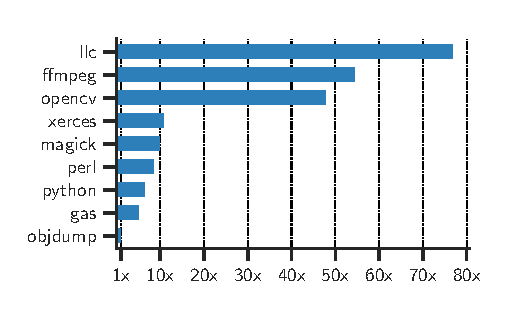
\includegraphics[clip, trim=0.47cm 0.4cm 0.45cm 0.65cm, width=0.8\columnwidth]{fig/objdump-size-comp}
	\caption{Comparing the code size of our subjects to \textsf{objdump} (code size about 339KB). Code size reported with GNU \textsf{size} utility.}
	\Description{Comparing the code size of our subjects to the size of objdump}
	\label{fig:code-size-comp}
\end{figure}


\subsection*{RQ2. Instrumentation Overhead}



% clip, left, bottom, right, top
\begin{figure*}[t!]
	\centering
	\small
	\begin{subfigure}[t]{0.29\textwidth}
		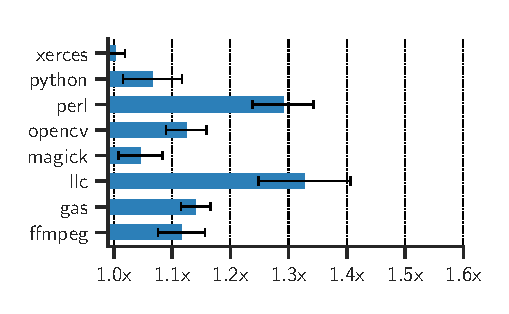
\includegraphics[clip, trim=0.48cm 0.4cm 1.4cm 0.65cm, width=\textwidth]{fig/perf-overhead}
		\caption{performance overhead}
		\label{fig:performance-overhead}
	\end{subfigure}
	\hspace{10pt}
	\begin{subfigure}[t]{0.29\textwidth}
		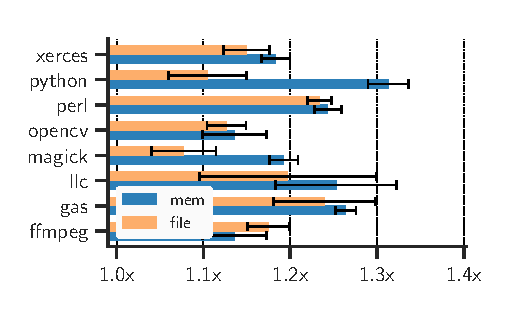
\includegraphics[clip, trim=0.47cm 0.42cm 1.65cm 0.65cm, width=\textwidth]{fig/any-overhead}
		\caption{size overhead}
		\label{fig:size-overhead}
	\end{subfigure}
	\hspace{10pt}
	\begin{subfigure}[t]{0.3\textwidth}
		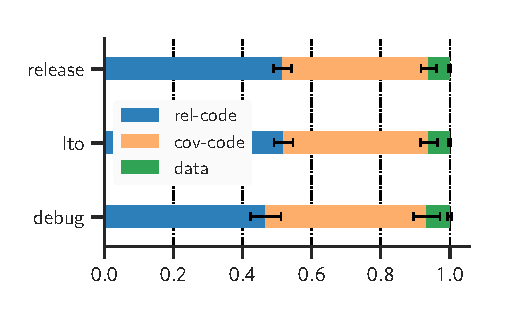
\includegraphics[clip, trim=0.48cm 0.36cm 0.75cm 0.65cm, width=\textwidth]{fig/overhead-dist}
		\caption{overhead distribution}
		\label{fig:overhead-dist}
	\end{subfigure}
	
	\caption{Overhead of the any-node instrumentation policy. (a) performance overhead accounts for instrumentation and dumping coverage data, (b) memory and file size overhead (c) distribution of memory overhead between code (relocated  and coverage update) and coverage data. }
	\Description{Overhead of the any-node instrumentation policy}
	\label{fig:overhead-results}
\end{figure*}



% clip, left, bottom, right, top
\begin{figure*}[t!]
	\centering
	\small
	\begin{subfigure}[t]{0.27\textwidth}
		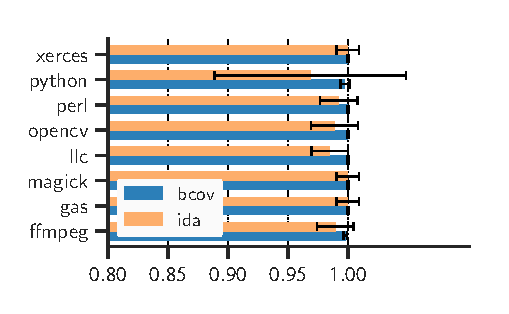
\includegraphics[clip, trim=0.48cm 0.4cm 1.71cm 0.65cm, width=\textwidth]{fig/jumptab-clang}
		\caption{\textsf{clang} binaries}
		\label{fig:jumptab-clang}
	\end{subfigure}
	\hspace{10pt}
	\begin{subfigure}[t]{0.28\textwidth}
		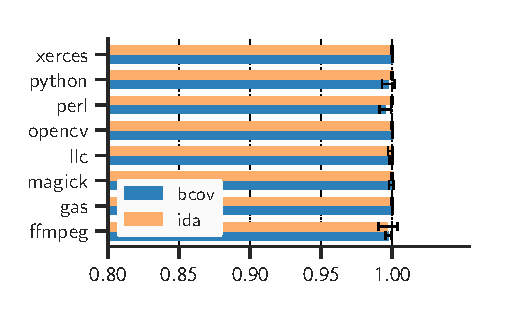
\includegraphics[clip, trim=0.48cm 0.4cm 1.6cm 0.65cm, width=\textwidth]{fig/jumptab-gcc}
		\caption{\textsf{gcc} binaries}
		\label{fig:jumptab-gcc}
	\end{subfigure}
	\hspace{10pt}
	\begin{subfigure}[t]{0.28\textwidth}
		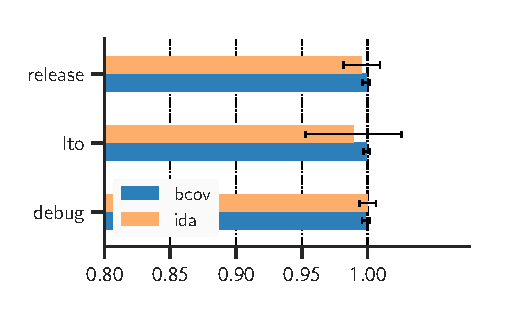
\includegraphics[clip, trim=0.48cm 0.38cm 1.6cm 0.8cm, width=\textwidth]{fig/jumptab-build}
		\caption{build type}
		\label{fig:jumptab-build-type}
	\end{subfigure}
	
	\caption{Normalized jump table analysis results in comparison to IDA Pro. \textbf{(a)} IDA Pro shows significant  variance on \textsf{clang} binaries. \textbf{(b)} both tools are comparable on \textsf{gcc} binaries. \textbf{(c)} varying the build type did not affect {\bcov}.}
	\Description{Normalized jump table analysis results in comparison to IDA Pro}
	\label{fig:jumptab-results}
\end{figure*}

Figure~\ref{fig:overhead-results} depicts the instrumentation overhead of the any-node policy relative to the original binaries. 
We omit the detailed evaluation of the leaf-node policy because of the lack of space.
The average performance overheads of the leaf-node and any-node polices are 8\% and 14\% respectively.
The overhead is measured based on the wall-clock time required to run individual test suites, .e.g, run ``\textsf{make test}'' to completion.
This covers the overhead associated with instrumentation and dumping coverage data to disk.
The latter overhead varies depending on the number of processes spawned during testing.

For example, all \textsf{opencv} tests are executed within a single process that dumps coverage data only once.
On the other hand, unit testing of \textsf{llc} spawns over 7,500 processes in about 40s.
This results in dumping $\sim$4\,GB of coverage data which significantly contributes to the overall delay.
Online merging of coverage data might reduce this disk IO overhead.
To give a better intuition, we note that without online merging, \textsf{llvm-cov} would dump over 320GB of coverage (and profiling) data for the same benchmark. 

To gain a better insight into the distribution of performance overhead, we experimented with the following variants of the any-node policy:

\begin{itemize}
	\item Detour only (DO). Here, we enabled only inserting detours and relocating overwritten instructions to the trampolines.
	\item Detour hosting (DH). Similar to DO, but we also enabled detour hosting for short basic blocks.
	\item Coverage update (CU). Similar to DH, but we also enabled inserting coverage update code in the trampoline. 
\end{itemize}

Note that the last variant is equivalent to the any-node policy.
We separately used each variant to patch all subjects in 4 different release builds.
Then, we ran their respective test suites to measure the performance overhead.
Interestingly, DO alone accounts for about 96\% of the overhead on average.
That is, DH and CU contributed only marginally.
This result suggests that inlining coverage update code, and thereby eliminating the need for trampolines,  may lead to substantial performance savings.

  
The average memory and file size overheads introduced by {\bcov} are 22\% and 16\% respectively.
We measure the memory overhead relative to the size of loadable ELF segments only. 
Recall that {\bcov} does not affect the run-time heap or stack.
The fact that other static instrumentation techniques need to duplicate the code segment~\cite{Anand:EuroSys2013,Laurenzano2010}, suggests that the overhead of {\bcov} is reasonable.
Coverage data represents only 6\% of the memory overhead.
It is worth noting that compiler optimizations can force {\bcov} to relocate more instructions.
This might be due to emitting smaller basic blocks.
However, our static instrumentation techniques are effective in reducing the difference in relocation overhead between debug and optimized builds as shown in Figure~\ref{fig:overhead-dist}.


\subsection*{RQ3. Jump Table Analysis}
Evaluating sliced microexecution requires comparing {\bcov} with representative binary analysis tools.
However, it was not possible to compare with BAP~\cite{BAP:CAV2011Brumley} and \textsf{angr}~\cite{angr:Shoshitaishvili2016} which are the leading academic tools.
BAP does not have built-in support for jump table analysis, while \textsf{angr} (v8.18.10) crashed on \textsf{opencv} and \textsf{llc} binaries.
For the remaining binaries, \texttt{angr} reported significantly fewer jump tables compared to IDA Pro.
Therefore, we compare {\bcov} only with IDA Pro (v7.2).
This should not affect our results since IDA~Pro is the leading industry disassembler.

Next, we have to establish the ground truth of jump table addresses --- specifically, the addresses of their indirect \texttt{jmp} instructions.
This is challenging as compilers do not directly emit such information.
Therefore, we conducted a differential comparison.
We observed that {\bcov} and IDA Pro agree on the majority of jump tables including their targets, so we manually examined the remaining cases where they disagree.
Both tools did not report false positives.
That is, they only missed jump tables.
This is expected in {\bcov} as repeated microexecution inspires high confidence in its results.
Therefore, our ground truth is the union of jump table addresses recovered by both tools.

Figure~\ref{fig:jumptab-results} depicts the recovery percentages relative to this ground truth consisting of over 46,000 jump tables.
We control for different factors affecting compilation.
We observed that IDA Pro delivers lower accuracy on \textsf{clang} binaries compared to \textsf{gcc} binaries, and its accuracy was affected by compiler optimizations.
In comparison, {\bcov} demonstrates higher robustness across the board.



\subsection*{RQ4. Comparison with DBI Tools}



\begin{table*}[t!]
	\centering
	\setlength\tabcolsep{8.5pt}
	\small
	\caption{Evaluating the accuracy of \textsf{bcov} based on \textsf{drcov} traces. 
    We show the number of processes spawned during testing, corresponding dump sizes in MB,
    and the total number of BBs and their instructions in original binaries.
    Both tools dump one coverage file per process.
    For each subject, we list the average/maximum of true positives (TP).
    FPs and FNs are also considered by listing the average precision and recall respectively.		 
    DR could not complete the test suite runs of \textsf{perl} and \textsf{python}.
    Omitted \textsf{opencv} as \textsf{drcov}'s data was invalid due to a bug. 
    }
    \label{tab:coverage-accuracy}        
	%    \renewcommand{\arraystretch}{1}
	\begin{tabularx}{0.99\textwidth}{@{}lllllllllll@{}}
        \\
		\textbf{Module} &
		\textbf{process \#} &
		\textbf{drcov size} &
		\textbf{bcov size} &
		\textbf{BB} &
		\textbf{Inst.} &
		\textbf{TP BB} &
		\textbf{TP Inst.} &
		\textbf{Precision} &
		\textbf{Recall} \\		
		\toprule
		
		xerces   & 80     & 12.34     & 4.32     & 116378   & 420096   & 9523.2~/~21927    & 40651.2~/~92144     & 99,98\%   &  99.42\%   \\ 
		magick   & 58     & 7.71      & 2.90     & 125521   & 521107   & 5689.4~/~20709    & 21614.9~/~83444     & 99,98\%   &  99.94\%    \\ 
		llc      & 7862   & 3481.97   & 4176.16  & 1067151  & 4343021  & 45184.5~/~90952   & 257209.5~/~461656   & 99,98\%   &  99.68\%  \\ 		
		gas      & 1235   & 71.94     & 38.56    & 60511    & 220447   & 2916.4~/~5015     & 11045.8~/~19578     & 99.93\%   &  99.67\%   \\ 
		ffmpeg   & 3309   & 423.45    & 762.39   & 496404   & 3050228  & 9682.0~/~14489    & 41439.1~/~63591     & 99.98\%   &  99.94\%   \\ 
		
		\bottomrule
	\end{tabularx}
\end{table*}


Pin and DynamoRIO (DR) are the most popular DBI tools.
Both act as a process virtual machine which instruments programs while JIT-emitting instructions to a code cache.
This complex process creates the following sources of overhead: 
(1) JIT optimization, and (2) client instrumentation.
To evaluate this overhead on our test suites, we installed the latest stable releases of both tools, namely, Pin v3.11 and DR v7.1.
We then replaced each of our subjects with a wrapper executable.
In the case of shared libraries, we replaced their test harness with our wrapper.
The test system would now run our wrapper, which in turn runs its corresponding original binary but under the control of a DBI tool. 
The wrapper reads a designated environment variable to choose between Pin and DR.

\cref{fig:dbi-tools-comparison} depicts the performance overhead of Pin and DR without client instrumentation.
It also shows the overhead of DR after enabling \textsf{drcov}, its code coverage client.
Note that Pin does not have a similar coverage client built-in.
The overhead is measured relative to original binaries and is averaged for four different release builds.
Both tools introduced regressions on \textsf{perl} and \textsf{python}.
However, DR made tests hung on \textsf{perl} and crashed on the \textsf{python} test suite. 
This highlights the challenges of maintaining transparency in DBI tools. 
Note that the DBI overhead of executable subjects is significantly higher than that of shared libraries. 
This can be attributed to the start-up delay which dominates in short-running tests.
The average performance overheads of Pin and DR are 29.1x and 4.1x respectively.
Enabling \textsf{drcov} increases the average overhead to 7.3x.
For the same benchmarks, {\bcov} introduced an average overhead of 11\% only.
Our experiments show that {\bcov} provides significantly better performance, transparency, and usability. 


% clip, left, bottom, right, top
\begin{figure}[t!]
    \centering
    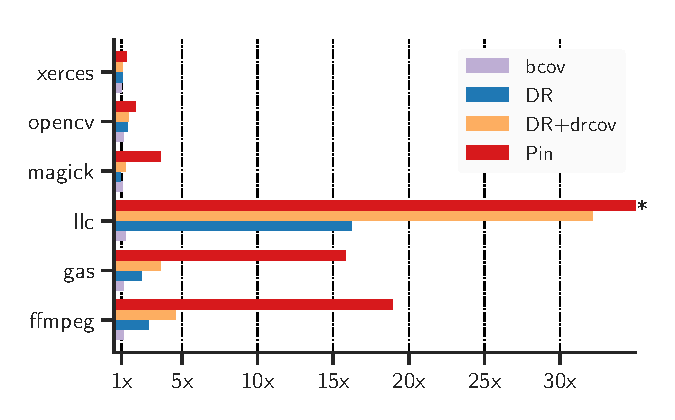
\includegraphics[clip, trim=0.48cm 0.4cm 0.49cm 0.73cm, width=0.9\columnwidth]{fig/dbi-overhead.pdf}
    \caption{Comparing the performance overhead of Pin, DynamoRIO (DR), \textsf{drcov}, and {\bcov}. Omitted \textsf{perl} and \textsf{python} as DR was  unable of completing their test suite runs. 
        (*) The actual overhead of Pin for \textsf{llc} is over 130x.}
    \Description{Comparing the performance overhead of Pin, DynamoRIO (DR)}
    \label{fig:dbi-tools-comparison}
\end{figure}


\subsection*{RQ5. Coverage Report Accuracy}
We evaluate the accuracy of the reported coverage by tracing binaries that are instrumented by {\bcov}. 
We use the any-node policy because of its precision.
Note that comparing the coverage of original binaries separately to instrumented ones will likely introduce errors that are only caused by non-determinism.
For example, repeatedly printing a simple: ``Hello World'' using \textsf{perl} will produce different instruction traces.



Initially, we obtained the ground truth traces using Intel~PT (IPT).
To this end, we collected about 2,000 sample tests from our test suites.
Running these tests produces 104GB of IPT data and 444MB of {\bcov} coverage data.
We used the standard \textsf{perf} tracing facilities in kernel v4.15 and later kernel v5.3.
We tried many IPT configurations and restricted ourselves to tests terminating in $ \le $ 5 seconds.
Despite these efforts, we could not reliably evaluate {\bcov} due to non-deterministic loss in IPT data. 
After all, disks might just be incapable of keeping up with the CPU~\cite{IntelPTLinuxDocs}.

We then turned to \textsf{drcov} to obtain the ground truth.
This DR client dumps the address of encountered basic blocks (BB) heads, i.e., first instruction.
We leverage the fact that our instrumentation does not modify BB heads.
Based on this, we expect BBs reported as covered by {\bcov} to appear in \textsf{drcov}'s trace.
We consider these BBs to be true positives (TP).
On the other hand, a BB reported by bcov that was not found in the trace represents a false-positive (FP). 
Similarly, a false-negative (FN) is a tracked BB that was missed by bcov. 
Both FPs and FNs represent errors in the reported coverage. 
Our evaluation method is conservative given the potential overapproximation in the CFG.
Also, we take into account the fact that \textsf{drcov} reports the heads of \textit{dynamic} BBs. 
This means that should A and B be consecutive BBs where A is fallthrough, i.e., does not end with a branch, 
\textsf{drcov} might only report the head of A.


Our results are shown in Table~\ref{tab:coverage-accuracy}.
They are based on running the test suites of subjects compiled with \textsf{gcc-7} in release build.
The results are representative of other build types.
The subjects are instrumented with {\bcov} and also run under the control of DR's \textsf{drcov}.
We list the average/maximum of TPs across all test processes. 
For example, the average number of TP BBs among 7,862 \textsf{llc} processes is 45,184.5, and the maximum is 90,952.
The average precision and recall across all subjects are 99.97\% and 99.95\% respectively.
This results in an average F-score of 99.86\%.
Our evaluation suggests that the reported coverage errors are practically negligible.
Nevertheless, there is still room for further improvement. 
Specifically, improving CFG precision and detour hosting can reduce FPs and FNs respectively. 

%Finally, we note that \textsf{drcov}'s traces preserve the transitions between basic blocks.
%This can provide more edge-level feedback signal in fuzzing. 
%This information is not available in our 
%On the other hand, \textsf{bcov} coverage data represent which might be useful 
%DR provides dynamic traces while we provide static traces.

%%% Local Variables:
%%% mode: latex
%%% TeX-master: "binder"
%%% End:
